\chapter{Anwendungen von Predictive Analytics im öffentlichen Sektor}

Zum Schluss werden einige Anwendungen von Predictive Analytics im öffentlichen
Sektor vorgestellt. Es wurden Anwendungsfälle in den Bereichen öffentliche Verwaltung,
Gesundheit und Bildung betrachtet. Zudem wurden zwei Fallstudien erstellt, bei denen
zwei konkrete Anwendungen besonders ausführlich untersucht wurden.

% TODO
% 2 grundlegende Probleme
% - Datenschutz: Achtung Privatsphäre + Angst vor Missbrauch
% - Verzerrungen in Daten: insb. auch Big Data, Daten nicht repräsentativ,
%     Daten kulturabhängig

\section{Öffentliche Verwaltung}

% TODO
% Daten in der öffentlichen Verwaltung
% Open Data Portale ( GovData.de )
% Abgrenzung zu 'Nowcasting'
% Predictive Policing
% Einschätzung der politischen Stimmungslage
% Vorhersage kultureller Unterschiede

% wackeligste Stimmen identifizieren und sie bei der Wahlwerbung zu priorisieren

% TODO Daten (-> Heise) 
% Thapa_Parycek S. 46

\subsection{Predictive Analytics in der Steuerverwaltung}

Die Anwendungen von Predictive Analytics in der Steuerverwaltung werden in einer
Studie des \emph{Forum on Tax Administration} (FTA) diskutiert\footnote{
Deutschland ist bei dieser Studie allerdings nicht dabei.
}. Der folgende Text beschreibt diese Anwendungsfälle.

\subsubsection{Audit Case Selection}

Steuerbehörden führen Kontrollen von Unternehmen und Personen durch, um Steuerbetrug
aufzudecken und zu verringern. Um verfügbare Ressourcen besser einzusetzen, werden mit Hilfe
von Predictive Analytics die Fälle für die Prüfung priorisiert, bei denen der größte Betrugsverdacht
besteht (Risikogruppen). Dieser Prozess wird als \emph{Audit Case Selection} bezeichnet und ist das hauptsächliche
Anwendungsgebiet von Predictive Analytics in der Steuerverwaltung (vgl. \cite{OECD}, S.~20).

Eine Besonderheit dabei ist die Analyse sozialer Netzwerke (\emph{Social Network Analysis}; \cite{OECD}, S.~21-22),
die zur Aufdeckung besonderer Formen von Einkommenssteuerbetrug eingesetzt wird. Die Analyse sozialer Netzwerke kann
Risikogruppen finden, die von Analysen auf individueller Ebene übersehen werden. Bei der Analyse werden die Beziehungen
zwischen Individuen erkennbar und können als visualisierte Netzwerke betrachtet werden. Die weitere Analyse dieser Netzwerke
kann durch Sachbearbeiter erfolgen oder mit Hilfe von regelbasierten oder statistischen Modellen durchgeführt werden.

\subsubsection{Payment Compliance}

Das Ziel der Payment Compliance ist es, ausstehende Zahlungen möglichst einzufordern oder das Problem gar nicht erst
entstehen zu lassen (vgl. \cite{OECD}, S.~24). Die typische Aufgabe von Predictive Analytics ist hierbei, die
Steuerzahler herauszufiltern, bei denen das größte Risiko besteht, dass sie ihre Zahlungsverpflichtungen nicht erfüllen werden. 
Eine weitere Anwendung, ist herauszufinden, wie am effektivsten mit dieser Gruppe kommuniziert werden kann (Prescriptive Analytics).

\subsubsection{Debt Management}

Beim traditionellen Debt Management werden Gruppen von Hochrisikoschuldnern identifiziert, um vorhandene Ressourcen auf sie zu
konzentrieren (vgl. \cite{OECD}, S.~26). Bei einer neueren Methode (\emph{Uplift Modelling}) werden Fälle selektiert, die
mit möglichst hoher Wahrscheinlichkeit auf eine Intervention seitens der Behörde reagieren werden. 

\subsubsection{Verbesserung der Serviceleistungen für Steuerzahler}

Text Mining (inklusive \emph{Sentiment Analysis}) kommt bei den Steuerbehörden zum Einsatz, um die Kommunikation mit den
Steuerzahlern zu verbessern (vgl. \cite{OECD}, S.~27). So werden beispielsweise ankommende E-Mails in Singapur mit Hilfe
von Text Mining bearbeitet, um die Art der Anfrage herauszufinden (vgl. \cite{OECD}, S.~27-28). In einem Fall konnte eine
Gruppe ähnlicher Anfragen identifiziert werden, nachdem eine Steuerrichtlinie verändert worden war. Die Behörde war dann in
der Lage frühzeitig zu reagieren und die Steuerzahler zusätzlich zu informieren. Text Mining hat in Singapur die manuelle
Bearbeitung von E-Mail Anfragen abgelöst. Dies ermöglicht eine objektivere Verarbeitung der Anfragen, da weniger Missverständnisse
entstehen. Zusätzlich wird die Arbeitszeit der Sachbearbeiter eingespart.

\subsubsection{Entscheidungsunterstützung}

Die meisten Datenanalysen bei den Steuerbehörden werden durchgeführt, um operative
Entscheidungen zu unterstützen (vgl. \cite{OECD}, S.~28). Allerdings exisitieren auch
Anwendungen, die strategische und politische Entscheidungen unterstützen. So werden
Analysen zur Abschätzung der Steuerlücke (\emph{tax gap analysis};vgl. \cite{OECD}, S.~28) durchgeführt.
Weiterhin wird versucht, den Einfluss von Änderungen in der Steuerpolitik vorherzusagen. Ein Beispiel
dafür, wenn auch streng genommen keine Predictive Analytics Anwendung, ist das ökonomische Modell, das
2012 von den chinesischen Behörden erstellt wurde, um die Effekte einer Steuerreform auf die Wirtschaft
und die soziale Wohlfahrt abzuschätzen (vgl. \cite{OECD}, S.~29). Der entsprechende Bericht der
Datenanalysten spielte eine wichtige Rolle in dem folgenden Reformprozess.

\subsubsection{Probleme mit Daten}

Der Bericht des FTA enthält auch eine Diskussion einiger Probleme, die im Zusammenhang mit Daten
festgestellt wurden.

So gibt es Bedenken, ob die gesammelten Daten, die anschließend für das Training der Modelle verwendet werden,
repräsentativ sind (vgl. \cite{OECD}, S.~51). Denn die verwendeten Daten stammen oft von stark verzerrten
Stichproben, wie beispielsweise alten Untersuchungsfällen. Somit wird nur ein kleiner Ausschnitt aus der
Gesamtpopulation zum Training der Modelle verwendet, was zu Selektionseffekten und schließlich zu Verzerrungen
im Modell führt. Um dieses Problem zu beheben, beziehen US-Steuerbehörden ihre Daten aus zufällig ausgewählten
Stichproben von Steuerprüfungen, um die Daten repräsentativer zu gestalten (vgl. \cite{OECD}, S.~52).

Weiterhin werden die Daten für Predictive Analytics Projekte eigentlich für operative Zwecke erhoben und
gespeichert (vgl. \cite{OECD}, S.~52). Aus diesem Grund ergeben sich verpasste Gelegenheiten, denn manche Daten, die nicht sinnvoll
für operative Zwecke sind, können nützlich für Datenanalysen sein. Zum Beispiel werden Beanstandungsgründe nach
einer Steuerprüfung typischerweise nicht gespeichert. Diese Information wäre jedoch hilfreich, um gesonderte Modelle
für verschiedene Beanstandungsgründe zu erstellen (vgl. \cite{OECD}, S.~52). 

\subsection{Predictive Policing}

Grafik aus \cite{Bode}, S.~2.

\begin{figure}%[!hbt]
\centering
\caption{Predictive Policing Prozess}
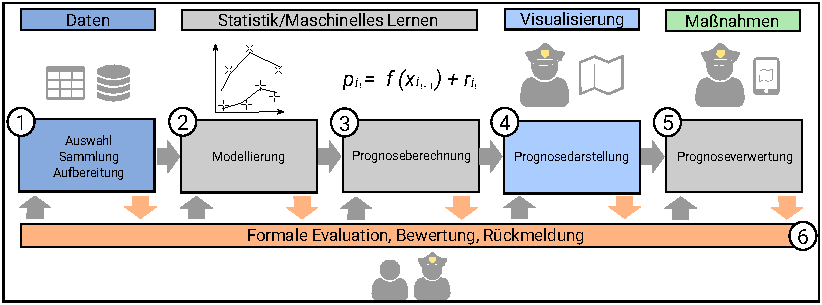
\includegraphics[scale=1.1]{Grafiken/Predictive_Policing_Ink.pdf} 
\label{pic:Predictive_Policing}
\end{figure}

\subsection{Wahlen und Parteiarbeit}

Ein bekannteres (und umstritteneres) Beispiel für die Anwendung von Datenanalysen
für politische und wahlkampftaktische Ziele ist der Fall von Cambridge Analytica.

\subsubsection{Cambridge Analytica - Fallstudie}

\begin{figure}%[!hbt]
\centering
\caption{Nutzung von Facebook Likes zur Vorhersage von Nutzerattributen}
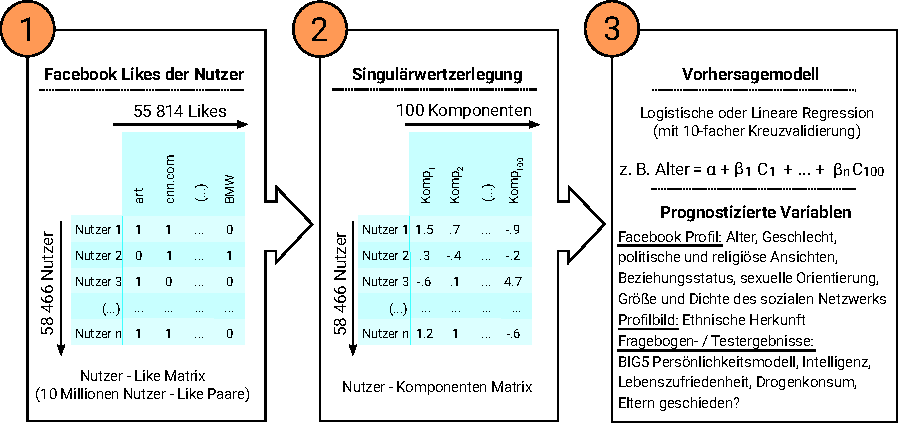
\includegraphics[scale=1.0]{Grafiken/Facebook_Likes_Ink.pdf} 
\label{pic:Like_Matrix}
\end{figure}

\section{Gesundheit}

Diese Haltung war überraschend genug, um eine Nachfrage des Journalisten
auszulösen.

% TODO
% Google Flu Trends (vorerst gescheitert)
% Kohortenstudien nützlich bei: bsp. Kampagnen zur öffentlichen Gesundheit
%   bsp. Ernährungskampagnen, Anti-Rauch-Kampagnen 
% Kohortenstudien: nicht persönlich (s. Watson, Abschnitt Cohort treatment),
%   aber Sicherheitsbedenken bleiben (Anonymisierung nicht möglich, Sicherheits
%   risiken ...)
\subsection{Flint Trinkwasserskandal - Fallstudie}

\section{Bildung}

% Anwendungsbeispiel Decision Tree
